% $Id: $
\documentclass[letterpaper,12pt,twoside]{book}
\usepackage[utf8]{inputenc}
\usepackage[spanish, es-tabla]{babel}
\usepackage{graphicx}
\usepackage{fix-cm} % scalable fonts
\usepackage{type1cm}
\usepackage{lettrine}
\usepackage{amssymb,amsmath,amsthm,amsfonts,latexsym}
\usepackage{wrapfig}
\usepackage{caption}
\usepackage[T1]{fontenc}
\usepackage[sc]{mathpazo}
%\usepackage{gb4e}
%\usepackage{gb4e}
\usepackage{extpfeil}
\usepackage[left=2.5cm,right=2.5cm]{geometry}
\usepackage{tikz}
\usetikzlibrary{arrows,shapes,trees,automata}
\usepackage{pgfplots}
\usepackage{float}
\usepackage{subfigure}
\usepackage{pifont}
%\usepackage{makeidx}
%\makeindex
\usepackage{tocbibind}
\usepackage{pdfpages}




\linespread{1.05}      
% Different font in captions
\newcommand{\captionfonts}{\small}

\makeatletter  % Allow the use of @ in command names
\long\def\@makecaption#1#2{%
 \vskip\abovecaptionskip
 \sbox\@tempboxa{{\captionfonts #1: #2}}%
 \ifdim \wd\@tempboxa>\hsize
   {\captionfonts #1: #2\par}
 \else
   \hbox to\hsize{\hfil\box\@tempboxa\hfil}%
 \fi
 \vskip\belowcaptionskip}
\makeatother   % Cancel the effect of \makeatletter



%\usepackage{mystyle_cgg}

%\usepackage{makeidx}
%\makeindex
%\usepackage[toc=true,hyper=true]{glossary}

%\makeglossary

\usepackage[round]{natbib} 
%%%%%%%%%%%%%%%%%%%
\newtheorem{definicion}{Definici\'on}
\newtheorem{ejemplo}{Ejemplo}
\newtheorem{teorema}{Teorema}
\newtheorem{lema}{Lema}
\newtheorem{prop}{Proposici\'on}
\newtheorem{af}{Afirmaci\'on}
\newtheorem{coro}{Corolario}
\newtheorem{obs}{Observaci\'on}
\newtheorem{casos}{Caso}
\renewcommand{\spanishrefname}{Bibliograf\'ia.}
\renewcommand{\spanishproofname}{Prueba.}
\decimalpoint
%\pagestyle{fancy}
\def\sectionautorefname{section}


%%%%%%%%%%%%%%%%

\begin{document}





% Use Roman numerals for table of contents etc.
\pagenumbering{roman}

\thispagestyle{empty}
\vspace{20 mm}
\begin{center}
\Huge
Ecuaciones Diferenciales\\
\Large Una introducción a la dinámica no lineal\\
      
\Large
\vspace{15mm}
\textsc{Pedro Miramontes}\\
Augusto Cabrera\\
Ulises Rayón\\
\Large
\large
Facultad de Ciencias\\
Universidad Nacional Aut\'onoma de M\'exico\\
\vspace{90 mm}
Ciudad de M\'exico\hspace{1mm}  \\
  
2020\\
\normalsize

\pagebreak
\thispagestyle{empty}
\vspace{20 mm}

 
\vspace{5 mm}
\large
Copyleft 2020 by \textsc{Pedro Miramontes, Augusto Cabrera y Ulises Rayón}\\
\normalsize
\vspace{10 mm}

\vspace{10 mm}
Todos los derechos de propiedad de esta publicaci\'on pertenecen a los autores
quienes otorgan su autorizaci\'on para que el lector pueda copiar,
imprimir o distribuir su trabajo libremente, en parte o en su totalidad, con las
\'unicas condiciones que: (i) El nombre del autor y el t\'itulo original deba ser citado en todo
momento, (iii) el texto no sea modificado y (iii) el uso de los
contenidos de esta publicaci\'on no sea comercial o con fines de lucro.\\



\vspace{60 mm}
Este libro ha sido producido electr\'onicamente con Software Libre
y acorde a una filosof\'ia de acceso libre para publicaciones acad\'emicas.
\end{center}

\newpage


\newpage


%\vspace*{3cm}

\chapter*{Pr\'ologo}





%%%%%%%%%%%%%%%%%%%%end of cover page
\newpage

\tableofcontents



\newpage






%\cleardoublepage
\chapter*{Agradecimientos}






%\newpage
\cleardoublepage

% Normal numbers for the rest of the thesis.
\pagenumbering{arabic}


\chapter{Notas históricas}
\addcontentsline{toc}{chapter}{Notas históricas}
\section{Historia}

Una ecuación diferencial es, antes de todo, una ecuación; es decir, una expresión matemática en la que aparecen elementos conocidos e incógnitas. Dichos elementos se encuentran a uno u otro lado de un signo de igualdad. Hay ecuaciones algebraicas

\[
\begin{aligned}
&\begin{array}{|c|c|c|}
\hline \multicolumn{2}{|c|} {\text { Ecuaciones diferenciales ordinarias }} & \text { Ecuaciones diferenciales parciales } \\
\hline \text { Clase } 1 & \text { Clase } 2 & \text { Clase } 3 \\
\hline
\end{array}\\
&\frac{d y}{d x}=f(y) \quad \hspace{8mm}\frac{d y}{d x}=f(x, y) \quad \hspace{20mm} x \frac{\partial u}{\partial x}+y \frac{\partial u}{\partial y}=u
\end{aligned}
\]



\cleardoublepage


\chapter{Ecuaciones diferenciales de primer orden}
\addcontentsline{toc}{chapter}{Ecuaciones diferenciales de primer orden}


\section{Procesos a tasa constante}

En la Naturaleza existe una gran cantidad de procesos que a lo largo del tiempo cambian o evolucionan a {\it tasa constante}. En esta sección haremos las definiciones esenciales y en las próximas veremos ejemplos de ellos.

Sin embargo, primero queremos precisar que cuando hablemos de {\it Naturaleza } entenderemos que comprende al mundo vivo --humano o no humano-- y los fenómenos que involucran a la materia inerte.

Vamos a  comenzar por lo básico. Supongamos que tenemos una magnitud $p(t)$ que es función del tiempo. Dicha magnitud puede representar a cualquier variable de interés de estudio: tamaño de una población, cantidad de dinero, número de enfermos, cantidad de material radioactivo, etcétera. Empezaremos por suponer que $p(t)$ solamente puede evaluarse en valores discretos del tiempo por lo cual es de interés estudiar la sucesión:
\[
\{p(t)\}_{t=0}^n = p(0),p(1),p(2)\hdots p(n)
\]
\noindent donde $n$ es un valor arbitrario del tiempo.

$p(n+1)-p(n)$ representa el incremento de la variable $p$ en una unidad de tiempo, mientras que:

 
\begin{equation} \label{eq:1}
 \dfrac {p(n+1) -p(n) }{p(n)}
\end{equation}

 
 Es el incremento de la magnitud $p$ con respecto a los existentes. Dado que el valor de un cociente no se altera si se multiplica por el mismo número su numerador y su denominador, se puede elegir un factor adecuado de manera que el denominador de la expresión \ref{eq:1} sea $100$ en cuyo caso diremos que se tiene  \emph{el incremento porcentual} o bien el \emph{incremento per cápita} de la magnitud $p(t)$ por unidad de tiempo. Si suponemos que el incremento porcentual es una constante $q$ es decir:
 
\begin{equation} \label{eq:2}
 \dfrac {p(n+1)-p(n)}{p(n)}=q
\end{equation}

\noindent Entonces el incremento por unidad de tiempo se puede expresar como: 

 \begin{equation} \label{eq:3}
 p(n+1) -p(n)=p(n)q
\end{equation}

De donde se deriva el hecho de que para medir el incremento de la magnitud $p$ en una unidad de tiempo, da lo mismo restar el valor futuro al actual que multiplicar el valor actual por la tasa de crecimiento porcentual por unidad de tiempo. Un despeje más nos lleva a:

 \begin{equation} \label{eq:4}
 p(n+1)=p(n)+p(n)q
\end{equation}

\noindent y arribamos a una verdad de perogrullo: el valor futuro de la magnitud $p(t)$ es igual a lo que se tenía más lo que aumentó. Más aún:

 \begin{equation} \label{eq:5}
 p(n+1)=p(n)(1+q)
\end{equation}

Entonces, el valor futuro es el valor anterior multiplicado por el factor $1+q$ que por esta razón recibe le nombre de \emph{tasa de reemplazo}.

Si ponemos $n=0$ y con la igualdad \ref{eq:5} calculamos $p(1)$ que, a su vez, nos sirve para calcular $p(2)$ y así sucesivamente. Llegamos la la expresión:

 \begin{equation} \label{eq:6}
 p(n)=p(0)(1+q)^n
\end{equation}

Esta es una \emph{fórmula predictiva}. Si se conoce la condición inicial $p(0)$ y la tasa de crecimiento \emph{per cápita} por unidad de tiempo, entonces la expresión \ref{eq:6} nos da la capacidad de conocer el valor futuro de $p$ para cualquier tiempo transcurrido mientras el tiempo se mida en unidades discretas.

\begin{ejemplo}
		
		
		\noindent La bacteria \emph{Escherichia coli} tiene una forma aproximadamente cilíndrica en la que la altura del cilindro mide cerca de 1$\mu$. Se reproduce por bipartición cada hora. La pregunta es ¿Sí se tiene inicialmente una bacteria, cuantas habrá después de una semana?.
		
		Si $p(0)=1$ y la unidad de tiempo es una hora, entonces $p(1)=2$ y, por lo tanto 
		 
\begin{equation} \label{eq:7}
 q=\dfrac{p(1)-p(0)}{p(0)}=\dfrac{2-1}{1}=1=\dfrac{100}{100}=100\%
\end{equation}

Una semana tiene 604800 segundos, por lo tanto y de acuerdo con nuestra fórmula predictiva \ref{eq:6}, dado que $q=1$ el resultado del ejercicio es:

\[
p(168)=2^{168}\approx 10^50
\]
Se deja al lector que realice el siguiente cálculo: si la bacteria fuera un cubo con $1\mu$ de lado ¿Qué volumen ocupan las bacterias que resultan de la reproducción a partir de una sola después de una semana?

\end{ejemplo}

\begin{ejemplo}

		\noindent La tasa de crecimiento de la República Mexicana en el 2015 fue 1.4\% anual. En ese mismo año la población total eran 9 millones. ¿Cuántos mexicanos habrá en el año 2050?
		
		En este caso $q=1.4\%=1.4/100=0.014$ y la $p(0)=9$. Donde hemos puesto el cero del tiempo en el 2015. Si ponemos que el tiempo transcurrido es de 35 años, la fórmula predictiva \ref{eq:6} queda como:
		
		\[
		p(35)=9\times(1.014)^{35}=9\times1.627=14.64 \textrm{ millones de habitantes}
		\]
		Esa es nuestra predicción. Sin embargo, la CONAPO pronostica una población de $7.7$ millones ¿Cómo explica usted la discrepancia?
		

\end{ejemplo}

En los dos ejemplos, tenemos sendas tasas de crecimiento positivas. Ahora vamos a ver que también se puede hablar de decrecimiento a tasa constante, veamos un ejemplo ilustrativo:

\begin{ejemplo}

\noindent  La cima del monte Everest se encuentra a $8,848$ metros sobre el nivel del mar y la presión atmosférica es de $0.33$ atmósferas. Se trata de encontrar la presión atmosférica en la Ciudad de México --$2240$ metros sobre el nivel del mar--.

En este caso, la variable independiente no es el tiempo sino la altura a partir del nivel de mar. A la altura cero la presión es $1$atm. 

\begin{align*}
  p(0) &= 1 \\
  p(8,848) &= 0.33p(0)
\end{align*}

Por lo tanto:

\[
q=\dfrac{p(1)-p(0)}{p(0)}=\dfrac{0.33-1}{1}=-0.66\%
\]

Es la tasa de decaimiento de la presión atmosférica por unidad de altura pero nos topamos con una dificultad técnica.La tasa $q$ que hemos calculado está definida cuando la unidad de altura es $1$ \emph{everest}. Desde luego que quisiéramos una tasa que estuviera, digamos, en metros. Vamos a ver que un razonamiento sencillo nos permitirá hacerlo:

\[
p(1)=p(0)(1+q_e)^1
p(1)=0.33p(O)
\]

Donde hemos llamado $q_e$ a la tasa medida en \emph{everests} pero debe de existir una tasa $q_m$ medida en metros que haga el mismo trabajo. Es decir;

\[
p(8,848)=p(0)(1+q_m)^{8,840}=0.33p(0)
\]
Usamos la segunda igualdad:


\begin{align*}
p(8,848) &=p(0)0.33\\
p(8,848) &=p(0)(1+q_m)^{8,848}
\end{align*}

Igualando los segundos términos y despejando la $q_m$, finalmente llegamos a:

\[
q_m=\sqrt[8848]{0.33}-1=0.0001259
\]



 Entonces, para saber la presión atmosférica en la Ciudad de México simplemente hay que calcular:

\[
p(2400)=p(0)(1+q_m)^{2400}=p(0)(1-0.0001259)^{2400}=p(0)0.76
\]

Y llegamos a la respuesta correcta: La presión atmosférica en la Ciudad de México es el $76\%$ de la presión al nivel del mar.

\end{ejemplo}



En el primer ejemplo nos daban como datos la población inicial y la población una unidad de tiempo después. En el segundo, se nos proporcionó la población inicial y la tasa de crecimiento. En el tercero aprendimos como calcular tasas de \emph{crecimiento equivalentes}. Esto va a resultar muy útil cuando queramos cambiar una tasa expresada en alguna unidad a la equivalente pero dada en submúltiplos de la unidad. Es un error muy común pero ampliamente usado en los medios de comunicación que si se tiene una tasa, digamos, anual, para obtener la tasa mensual se divide entre doce y ya. 

Si suponemos que tenemos un proceso que crece a la tasa de $q=120\%$ anual y nos dejamos guiar por los que leen las noticias, responderemos que la tasa mensual es del $10\%$

Llamemos $q_m$ a la tasa mensual equivalente y procedamos según lo ilustrado en el ejemplo número $3$: 

\begin{align*}
p(1)=p(0)(1+q)=p(0)(2.2)\\
p(12)=p(0)(1+q_m)^{12}=p(0)(2.2)
\end{align*}

Igualando las dos expresiones y siguiendo el procedimiento del ejemplo 3, se tiene que:

\[
q_m=\sqrt[12]{1+q}=\sqrt[12]{2.2}
\]

En nuestro caso $q=1.2$ por lo que después de hacer las cuentas llegamos a:

\[
q_m=0.0679
\]

De manera que la respuesta correcta es que la tasa mensual equivalente a una tasa anual del $120\%$ es del $6.79\%$. Por favor, verifíquelo. Es claro que sería un ejercicio inútil tratar de explicarlo a comentadores de noticias.

En un resumen parcial rápido, podemos decir que hemos aprendido lo que es una tasa de crecimiento per cápita y por unidad de tiempo. Tenemos la fórmula $6$ que es una poderosa herramienta de predicción siempre y cuando se mantenga firme la premisa de que \emph{la tasa sea constante}. También sabemos cómo proceder si conocemos la tasa $q$ para una unidad de tiempo (o más general; para una unidad de la variable independiente) y deseamos conocer la tasa equivalente para una subunidad. 

Si se conocen: i) La tasa de crecimiento $q$, ii) la condición inicial $p(0)$ y las unidades de tiempo $n$ que han de transcurrir, entonces podemos predecir el valor de la magnitud $p(n)$. A este esquema de trabajo, le vamos a llamar el \emph{problema directo}.

Sin embargo, también es un problema de importancia práctica el preguntarse cuántas unidades de tiempo $n$ han de transcurrir para que tengamos un valor prefijado de la magnitud $p(n)$

\begin{ejemplo}

Si la presión atmosférica disminuye con la altura a tasa constante ¿A qué altura se tendrá el $80\%$ de la presión al nivel del mar?
Recordemos la fórmula predictiva \ref{eq:6}

 \begin{equation*} 
 p(n)=p(0)(1+q)^n
\end{equation*}

Ahora la incógnita es la variable independiente $n$ mientras que los datos son la tasa $q_m$ (recordar la notación del ejemplo 3), la condición inicial $p(0)$ y la magnitud $p(n)$. Despejemos $n$ de la expresión anterior:

\[
n=\dfrac{\log\frac{p(n)}{p(0)}}{\log(1+q_m)}
\]

Y dado que sabemos que $q_m=0.01259$ y que $p(n)=0.8p(0)$, haciendo las sustituciones pertinentes\footnote{De aquí adelante utilizaremos la notación $\log()$ para el logaritmo natural. Todos los resultados son aproximados pues hemos truncado las los números a pocas cifras después del punto decimal.} llegamos a la respuesta: $n=1780.5135$. A la altura aproximada de $1780$ metros, la presión atmosférica es el $80\%$ de la que hay al nivel del mar.

\end{ejemplo}

Hasta ahora, todo parece ir sobre ruedas pero el ejemplo anterior amerita una mayor reflexión. El resultado de ls operaciones es $n=1780.5135$ y arbitrariamente nos hemos conformado con la aproximación truncando las cifras no enteras ¿Realmente no lo podemos hacer mejor?. 

Regresemos a la fórmula predictiva \ref{eq:6}: 

\[
p(n)=p(0)(1+q)^n
\]

En los párrafos anteriores insistimos en la variable independiente $n$ tenía que ser un número entero de modo que no podemos apostar a que la respuesta del ejemplo anterior sea rigurosamente la obtenida. Sin embargo, ya hemos desarrollado un método para encontrar la tasa de crecimiento per cápita para submúltiplos de la tasa por unidad de tiempo. Ahora supongamos que existe un número $k$, al que llamaremos la \emph{tasa instantánea} de crecimiento que cumple:

\begin{align}
    p(t)=p(0)(1+q)^t=p(0)e^{kt}
\end{align}

Que sea válida para $t$ entero pero que interpole los valores de $p(t)$ para cualquier valor de $t$ en los números reales. Si se conoce la tasa $q$ por unidad de tiempo, entonces es fácil calcular la tasa instantánea $k$



\section{El crecimiento Malhusiano}









\section{La separación de variables}

Para la ecuación del crecimiento malthusiano utilizamos que la ecuación $\dfrac{\mathrm{d}X}{\mathrm{d}t}=\rho X$ es equivalente a 
$$\int \dfrac{\mathrm{d}X}{X}=\int \rho\mathrm{d}t$$
Esta idea es una técnica estándar para resolver cierta clase de ecuaciones, llamadas de variables separadas, veamos algunos ejemplos antes de dilucidar por qué funciona el truco de la separación de variables.

\begin{ejemplo}
Consideremos la ecuación $\dfrac{\mathrm{d}Y}{\mathrm{d}X}=-\dfrac{X}{Y}$ esta ecuación diferencial es equivalente a la ecuación integral 
$$
\int Y\mathrm{d}Y =-\int X\mathrm{d}X
$$
integrando formalmente tenemos
$$
Y^2+X^2=\xi
$$
para alguna constante no-negativa $\xi$, las soluciones de este problema son círculos de radio $\xi$ .
\begin{figure}[H]
    \centering
    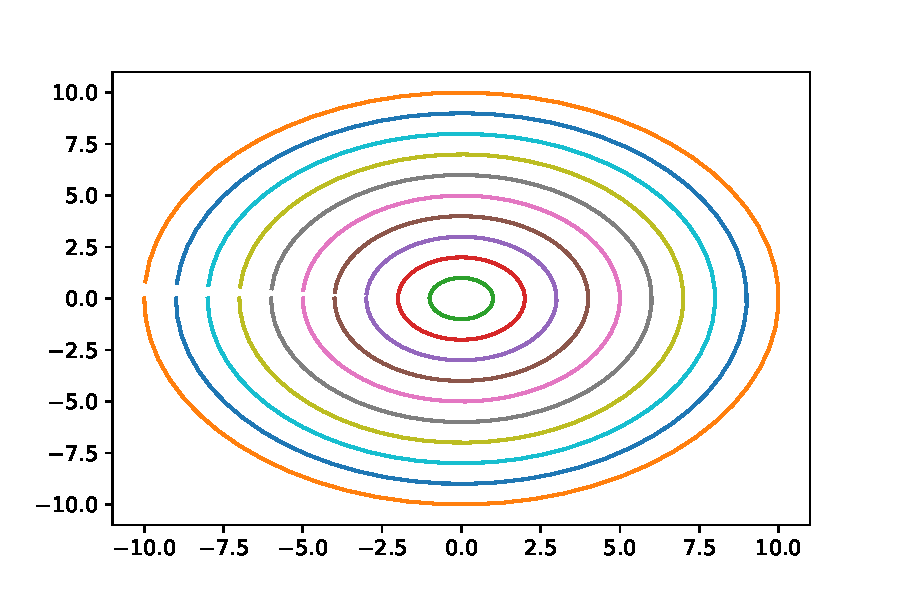
\includegraphics[scale=0.85]{circulos.pdf}
    \caption{Soluciones para el problema $\dfrac{\mathrm{d}Y}{\mathrm{d}X}=-\dfrac{X}{Y}$ }
    \label{fig:circ}
\end{figure}
\end{ejemplo}

\begin{ejemplo}
Consideremos la ecuación $\dfrac{\mathrm{d}Y}{\mathrm{d}X}=\dfrac{Y}{X}$ esta ecuación diferencial es equivalente a la ecuación integral 
$$
\int \dfrac{\mathrm{d}Y}{Y} =-\int \dfrac{\mathrm{d}X}{X}X
$$
integrando formalmente tenemos
$$
\ln(Y)=\ln(X)+\xi
$$
es decir
$$
Y(X)=e^{\xi}X
$$
\begin{figure}[H]
    \centering
    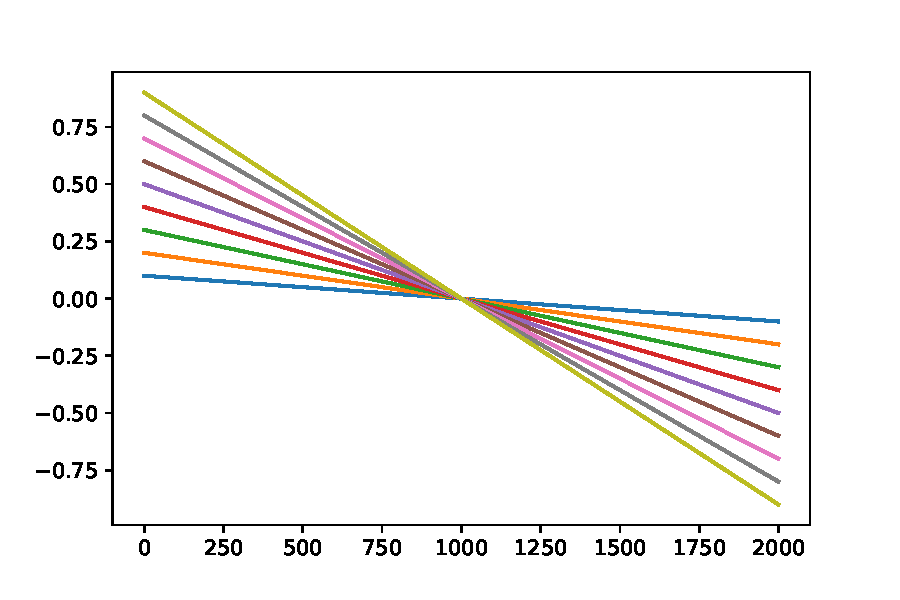
\includegraphics[scale=0.85]{ejemplo2.pdf}
    \caption{Soluciones para el problema $\dfrac{\mathrm{d}Y}{\mathrm{d}X}=\dfrac{Y}{X}$ para distintas condiciones iniciales}
    \label{fig:ej2}
\end{figure}
\end{ejemplo}
 
 Las ecuaciones que están dadas en la forma $\dfrac{\mathrm{d}Y}{\mathrm{d}X}=\dfrac{\Psi(X)}{\Phi(Y)}$ son llamadas de variables separadas, suponiendo que $\Psi$y $\Phi$ son continuas en el dominio correspondiente, entonces la ecuación integral
 $$
 \int\Phi(Y)\mathrm{d}Y=\int\Psi(X)\mathrm{d}X+\xi
 $$
 Esta ecuación integral es llamada finita (¿Se imagina por qué?) y también la satisfacen las soluciones de la ecuación diferencial. Una función de la forma $\Omega(x,y)=0$ que determina a $Y(X)$ como función implícita es llamada integral de la ecuación diferencial, si además esta función determina sin excepción  a todas las soluciones de la ecuación se llama una integral general.
 
 Si $Y(X_0)=Y_0$ es una condición inicial, entonces la integral
 $$
 \int_{Y_0}^{Y}\Phi(Y)\mathrm{d}Y=\int_{X_0}^{X}\Psi(X)\mathrm{d}X
 $$
determina de manera unívoca la solución.

\begin{figure}[H]
    \centering
    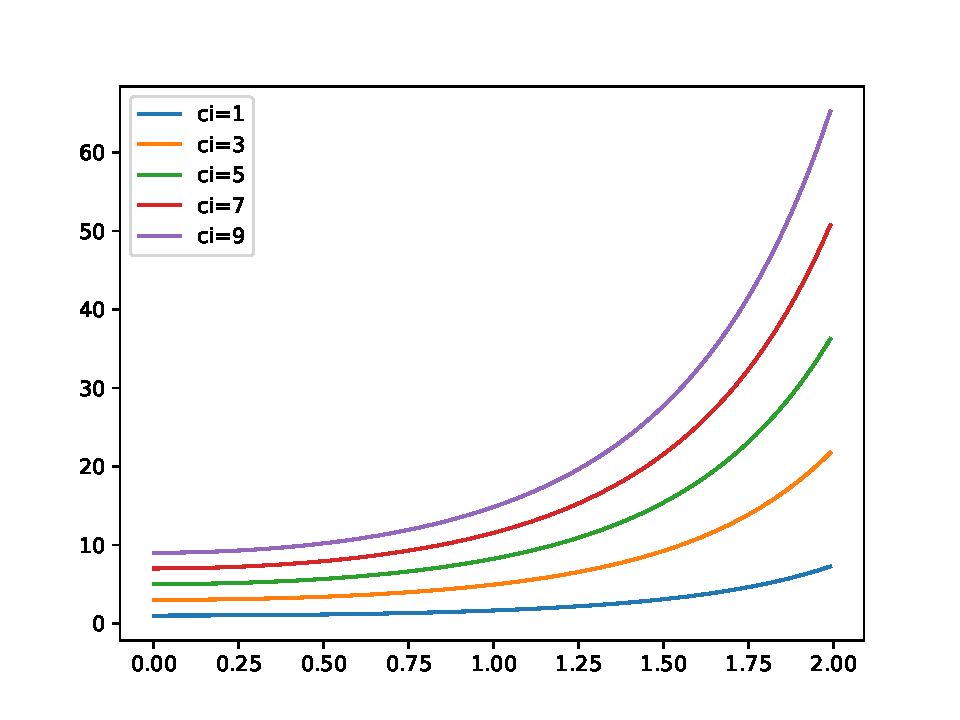
\includegraphics[scale=0.85]{exponenciales1.pdf}
    \caption{Soluciones de la ecuación de Malthus para distintos valores iniciales}
    \label{fig:exposci}
\end{figure}

Dada una condición inicial, para el problema del crecimiento exponencial, hay una solución única, para un valor fijo del parámetro $\rho$, ahora variaremos un poco este parámetro. Tenemos el siguiente comportamiento. 
\begin{enumerate}
    \item Para $\rho=0$ la solución es constante, en general una solución constante es llamada estacionaria.
    \item Para $\rho > 0$ El modelo describe u8n crecimiento ilimitado.
    \item Para $\rho<0$ El modelo describe un decrecimiento asintótico a cero. Podemos representar el cambio cualitativo de las soluciones cuando variamos  el parámetro mediante la llamada linea fase.
\end{enumerate}

\begin{figure}[H]
    \centering
    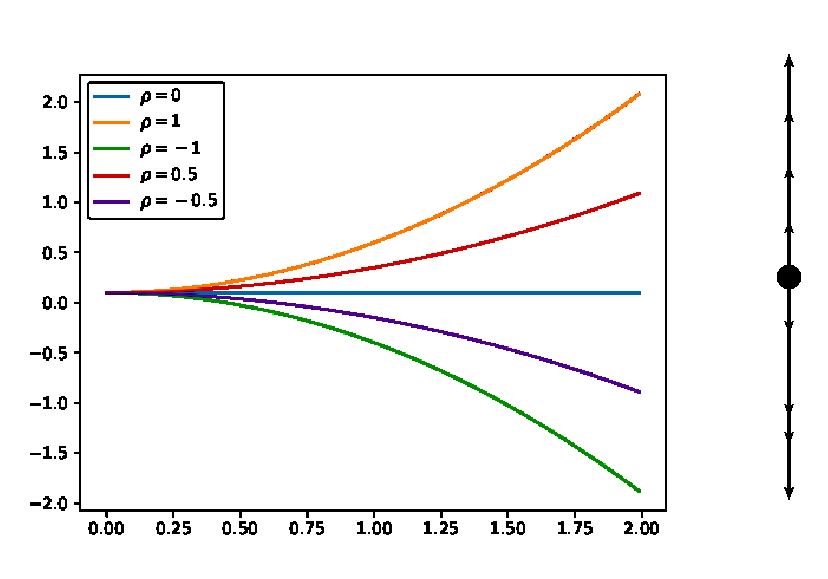
\includegraphics[scale=0.85]{exponenxiales2.pdf}
    \caption{distintos valores para el parámetro $\rho$}
    \label{fig:exposrho}
\end{figure}


Ahora pensemos en la siguiente ecuación:
$$
\varphi_1(x)\psi(y)\mathrm{d}x=\varphi_2(x)\psi_2(y)\mathrm{d}y
$$
no es una de variables separadas. Ahora si tenemos garantizado que : $\varphi_2(x)\neq 0$ y $\psi_2(y)\neq 0$, podemos  considerar la ecuación equivalente
$$
\frac{\varphi_1(x)}{\varphi_2(x)}\mathrm{d}x=\frac{\psi_1(y)}{\psi_2(y)}\mathrm{d}y
$$
que si es de variables separadas. A este tipo de ecuación se le llamda de variables separables.

Ahora hagamos un par de ejemplos sencillos:

\begin{ejemplo}
Consideremos la ecuación

$$
x(1+y^2)\mathrm{d}x-y(1+x^2)\mathrm{d}y=0
$$
está garantizado que  tanto $1+y^2$ como $1+x^2$ son estríctamente positivos, así que nuestra ecuación es equivalente a la ecuación de variables separadas
$$
\frac{y}{1+y^2}\mathrm{d}y=\frac{x}{1+x^2}\mathrm{d}x
$$
que a su vez es equivalente a la ecuación integral
$$
\int \frac{y}{1+y^2}\mathrm{d}y=\int \frac{x}{1+x^2}\mathrm{d}x
$$
cuya solución es 
$$
\ln(1+y^2)-\ln(1+x^2)=\xi
$$
y finalmente, tomando exponencial en ambos términos de la ecuación
$$
\frac{1+y^2}{1+x^2}=e^{\xi}=\zeta
$$
\end{ejemplo}

\begin{ejemplo}
La ecuación
$$
\dot{x}=4t\sqrt{x}
$$
con condición inicial $x(1)=1$ es de variables separables puesto que $\sqrt(x)$ no se anula si empezamos en $1$. Nuestra ecuación es equivalente a:
$$
\frac{\mathrm{d}x}{2\sqrt{x}}=2t\mathrm{d}t
$$
así que
$$
\int_{1}^{x}\frac{\mathrm{d}\xi}{2\sqrt{\xi}}=\int_{1}^{t}2\tau\mathrm{d}\tau
$$
y finalmente
$$
x(t)=t^4
$$
\end{ejemplo}
\section{Un modelo de poblaciones más realista}

En la primera sección vimos que el modelo propuesto por Malthus  además de ser políticamente malintencionado, es a todas luces equivocado, ninguna población puede crecer permanente e ilimitadamente. Cualquier población ve acotado su crecimiento por cierta ``presión'' ejercida por el ambiente. ¿Cómo modelamos esta ``presión''? El problema es ahora proponer un modelo para una población cuyo crecimiento quede acotado por su propia dinámica. Llamemos $K$ a tal presión ambiental, en la literatura se le llama capacidad de carga del sistema, representa la cantidad de individuos de cierta población, a los que el medio puede proveer de subsistencia. Nuevamente consideraremos que la tasa intrínseca (natural) de crecimiento de la población es $\rho$ y que el crecimiento es proporcional no sólo al tamaño de la población actual, sino que decrece proporcionalmente a la proporción entre la población actual y la capacidad de carga.

\begin{equation}
    \dot{x}=\rho(1-\frac{x}{K})x
\end{equation}

Lo primero que debemos notar es que esta ecuación ya no es lineal en $x$, tiene un término cuadrático que de alguna forma nos da información sobre las interacciones intraespecíficas de la población. Ahora busquemos las soluciones de equilibrio, es decir aquellas para las cuales no hay cambios en la población. En este caso es claro que cuando $x=0$ ó $\left(1-\dfrac{x}{K}\right)=0$, entonces $\dot{x}\equiv 0$. Al caso  $x=0$ lo llamaremos el equilibrio trivial, y corresponde a que no hay ningún cambio en la población, cuando   $\left(1-\dfrac{x}{K}\right)=0$ tenemos que $x\equiv K$, es decir que al alcanzar la capacidad de carga del sistema el crecimiento se detiene. 

Consideremos la función polinomial $x\mapsto \rho(1-\frac{x}{K})x$ es una cuadrática cóncava en la dirección negativa del eje $\mathrm{Y}$, que cruza al eje horizontal en los puntos $(0,0)$ y $(0,K)$ el punto máximo de la parábola $\rho x-\rho \dfrac{x^2}{K}=0$ se alcanza cuando $\rho-2\rho \dfrac{x}{K}=0$ o equivalentemente $x=\dfrac{K}{2}$, así para distintos valores de $K$, el máximo de la parábola está más o menos alejado de la gráfica de la identidad. Las soluciones de la ecuación se alejan del $(0,0)$ y se aproximan a $(0,K)$. 

Nótese que si la condición inicial es menor que el parametro $K$, entonces . Ahora si iniciamos en una condición $x_0 > K$ entonces el cociente $\dfrac{x_0}{K}>1$ y la derivada $\dot{x} < 0$ y por lo tanto las soluciones son decrecientes y en ambos casos se aproximan asintóticamente a $x\equiv K$, en efecto tomamos el límite

Ahora analicemos el caso más sencillo. Tomamos $K=1$. Si aplicamos el truco de la separación de variables, tenemos la ecuación integral

\begin{equation}
    \int \frac{\mathrm{d}x}{x(1-x)}=\rho\int\mathrm{d}t
\end{equation}
resolviendo por fracciones parciales tenemos
$$
\int\frac{\mathrm{d}x}{x}+\int\frac{\mathrm{d}x}{1-x}=\rho x +\xi_0
$$
tenemos que:
$$
\ln(\frac{x}{(1-x)}=\rho t+\xi_1
$$
se sigue que:
$$
x(t)=\xi\frac{e^{\rho t}}{1+e}
$$
\section{Teoremas de existencia y unicidad de las soluciones}

La clase de las ecuaciones diferenciales ordinarias que son integrables por cuadraturas es muy limitada, por ello la mayor\'ia de las ecuaciones se resuelve usando m\'etodos de aproximaci\'on num\'erica.


\begin{teorema}
Si en la ecuaci\'on
$$
\dfrac{\mathrm{d}f}{\mathrm{d}t}=f(x,y)
$$
la funci\'on
$f$ es continua en $D=\left[x_0-a,x_0+a\right]\times\left[y_0-b,y_0+b\right]$, adem\'as $f$ es Lipschitz-continua en $D$, es decir que existe una constante $N$ tal que $|f(x_1,y_1)-f(x_2,y_2)|\leq N|y_1,y_2|$ para $(x_i,y_i)\in D$.

Entonces existe una soluci\'on \'unica $y=\bar{y}(x)$ en el intervalo $\left[x_0-H,x_0+H\right]$ que satisface $y(x_0)=y_0$ y donde $H<\min\{a,\frac{b}{M},\frac{1}{N}\}$, $M=\max_{D}\{|f(x,y)|\} $
\end{teorema}


Las condiciones del teorema  requieren aclaraci\'on. La soluci\'on para la ecuaci\'on, que satisface las condiciones iniciales  existe s\'olo para $x\in [x_0-a,x_0+a]$ pero $y$ puede existir fuera del rect\'angulo $D$. Es decir $y=y_0\pm b$ para alg\'un $x=x_1\in[x_0-a,x_0+a]$. Si $x_1>x_0$ para $x>x_1$, la soluci\'on puede no estar definida.

Podemos garantizar que $y=\bar{y}(x)$ no se sale de $D$ cuando $x\in[x_0-H,x_0+H]$ con $H<a$ y $H<\frac{b}{M}$, $M=\tan\alpha$. Donde $\alpha$ es el coeficiente angular de latangente a la curva integral buscada. Si estas rectas se salen de $D$ entonces las absisas de los puntos de corte son $x_0\pm\dfrac{b}{M}$. As\'i la absisa  del punto de salida de lacurva inegral de $D$ puede solamen
te ser menor o igual que $x_0+\frac{b}{M}$ y mayor o igual que $x_0-\frac{b}{M}$. Puede mostrarse la existencia  dela soluci\'on en $[x_0-H,x_0+H]$ con $H=\min\{a,\frac{b}{M}\}$ pero ser\'a m\'as sencillo mostrarlo para $H<\min\{a,\frac{b}{M},\frac{1}{N}\}$

\begin{figure}[H]
\centering
\begin{tikzpicture}
\draw[](-0.3,0)--(6,0);
\draw (1,5)--(5,5);
\draw (1,5)--(1,2);
\draw (5,2)--(5,5);
\draw (1,2)--(5,2);
\draw[](0,-0.3)--(0,6);
\draw (1.3,2)to[bend left](3.5,3.5);
\filldraw (3.5,3.5) circle (2pt) ;
\draw (3.5,3.5)to[bend right](4.8,5);
\draw[dotted](3.5,3.5)--(3.5,0) node[pos=1.14]{$x_0$};
\draw[dotted](3.5,3.5)--(0,3.5) node[pos=1.1]{$y_0$};
\draw[dotted](1,5)--(1,0) node[pos=1.1]{$x_0-a$};
\draw[dotted](5,2)--(5,0) node[pos=1.2]{$x_0+a$};
\draw[dotted](1,5)--(0,5) node[pos=1.5]{$y_0+a$};
\draw[dotted](5,2)--(0,2) node[pos=1.1]{$y_0-a$};
\end{tikzpicture}
    \caption{}
    \label{fig:my_label}
\end{figure}

\begin{figure}[H]
    \centering
    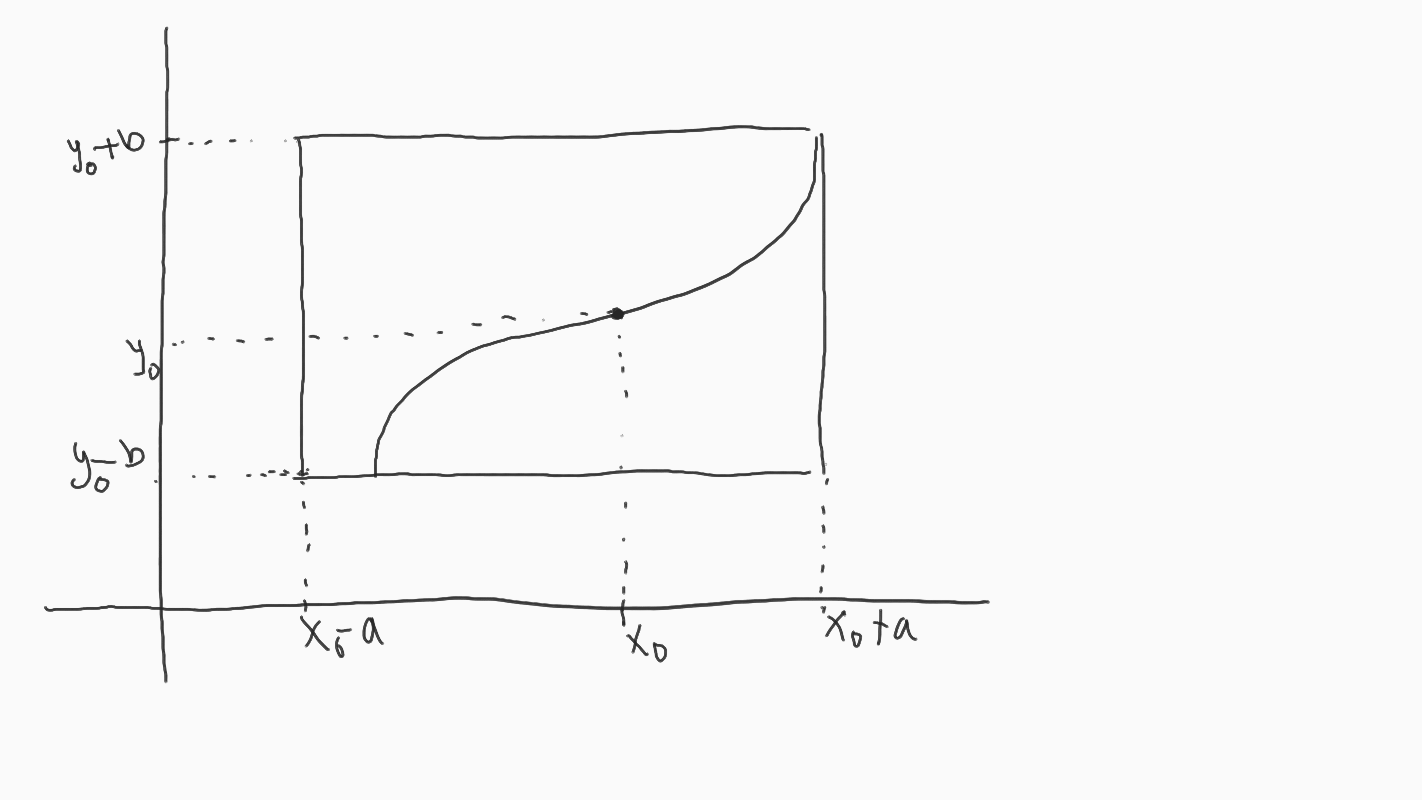
\includegraphics[scale=0.25]{graficas1.png}
    \caption{Caption}
    \label{fig:my_label}
\end{figure}


La condici\'on de Lipschitz 
$$
|f(x_1,y_1)-f(x_2,y_2)|\leq N(y_1-y_2)
$$
puede ser sustituida por otra m\'as fuerte, pero m\'as f\'acilmente comprobable, la existencia de $\partial_{y} f^{'}$ en $D$ y que sea acotada.

En efecto para $(x,y)\in D$ y $|f'_y(x,y)|\leq N$ entonces por el teorema del valor intermedio:
$$
|f(x_1,y_1)-f(x_2,y_2)|=|f'_y(x,\xi)|-|y_1-y_2| 
$$
con $\xi\in (y_1,y_2)$. As\'i $(x,\xi)\in D$ y $|f_y(x,\xi)|\leq N$ , $|f(x,y_1)-f(x,y_2)|\leq N|y_1-y_2|$.

\begin{proof}
Observemos primero que 
$$
\left.\begin{array}{cc}
    \dfrac{\mathrm{d}y}{\mathrm{d}x}&=f(x,y)  \\
    &\\
    y(x_0) &=y_0 
\end{array}\right.
$$
es equivalente a
$$
y=y_0+\int_{x_0}^xf(x,y)\mathrm{d}x
$$

En efecto:
$$
\int_{x_0}^x\frac{\mathrm{d}y}{\mathrm{d}x}\mathrm{d}x=\int_{x_0}^xf(x,y)\mathrm{d}x
$$
así
$$
y(x)-y(x_0)=\int_{x_0}^xf(x,y)\mathrm{d}x
$$
y por tanto
$$
y(x)=y_0+\int_{x_0}^xf(x,y)\mathrm{d}x
$$
Ahora, hagamos una aproximaci\'on de  la soluci\'on usando Euler
$$
y=y_n(x)
$$
con paso $h_n=\frac{H}{n}$ en $[x_0,x_0+H]$.

La poligonal asociada a la aproximaci\'on de Euler no sale de la regi\'on $D$ pues el coeficiente angular de cada segnmento es menor  que $M$ en m\'odulo.

A continuaci\'on probaremos que
\begin{enumerate}
\item la sucesi\'on  $(y_n)$ converge uniformemente.
\item $\bar{y}(x)=\lim_{n\rightarrow infty}y_n$ es soluci\'on para la ecuaci\'on integral.
  \item La soluci\'on es \'unica
\end{enumerate} 

Probemos $\bf{(1)}$. En efecto $y'_n(x)=f(x_k,y_k)$ 
\end{proof}
 
\cleardoublepage


\chapter*{Sistemas lineales}
\addcontentsline{toc}{chapter}{Sistemas lineales}
%\include{03-sistemas}




\chapter*{Sistemas no lineales}
\addcontentsline{toc}{chapter}{Sistemas no lineales}
%\include{04-nolineales}

\cleardoublepage








\end{document}


